\documentclass[../../General.tex]{subfiles}
\begin{document}

\section{Arquitectura eléctrica del sistema}

La integración del hardware para el prototipo de inspección se estructura a partir de la segregación funcional de las líneas de potencia y los buses de intercambio de datos, como se ilustra en la Figura \ref{fig:DiagramaBloques}. La fuente de energía primaria consiste en un paquete de baterías de iones de litio gestionado por un circuito supervisor de protección. Desde esta línea central, la energía se canaliza hacia convertidores reductores conmutados y reguladores lineales que acondicionan los potenciales requeridos por los distintos circuitos, manteniendo una separación galvánica y funcional para aislar el ruido eléctrico originado por la conmutación de los actuadores respecto a las etapas de sensado y control.

En el nivel de procesamiento y toma de decisiones, el controlador SBC actúa como el nodo maestro del vehículo. Mediante sus interfaces digitales, centraliza la conexión con los dispositivos periféricos principales, gestionando el módulo de comunicaciones de largo alcance por canal serial asíncrono, la recepción de coordenadas de navegación satelital y el almacenamiento en memoria microSD. A su vez, esta unidad adquiere los datos de la instrumentación meteorológica externa mediante buses RS-485 conectados a sus puertos USB y se enlaza con el microcontrolador mediante un puerto de comunicación serial entre dispositivos.

El microcontrolador asume la gestión de bajo nivel, ejecutando la lectura de la unidad de medición inercial y del monitor de energía mediante el bus I2C, la adquisición de señales del codificador rotativo incremental a través de líneas de interrupción, el estado de los interruptores de fin de carrera mediante entradas digitales y la temperatura del chasis mediante su módulo ADC. De manera complementaria, esta unidad genera los trenes de pulsos y señales de dirección para los controladores de los motores de elevación y orientación, las señales PWM para el puente completo del motorreductor de tracción en el eje posterior y los pulsos temporizados para los servomotores de dirección en el eje frontal.

\begin{figure}[H]
    \captionsetup{justification=raggedright, singlelinecheck=false, labelsep=none}
    \caption[Diagrama de bloques representativo de la arquitectura eléctrica.]{} 
    \textit{Diagrama de bloques representativo de la arquitectura eléctrica.} \par\medskip
    \centering
    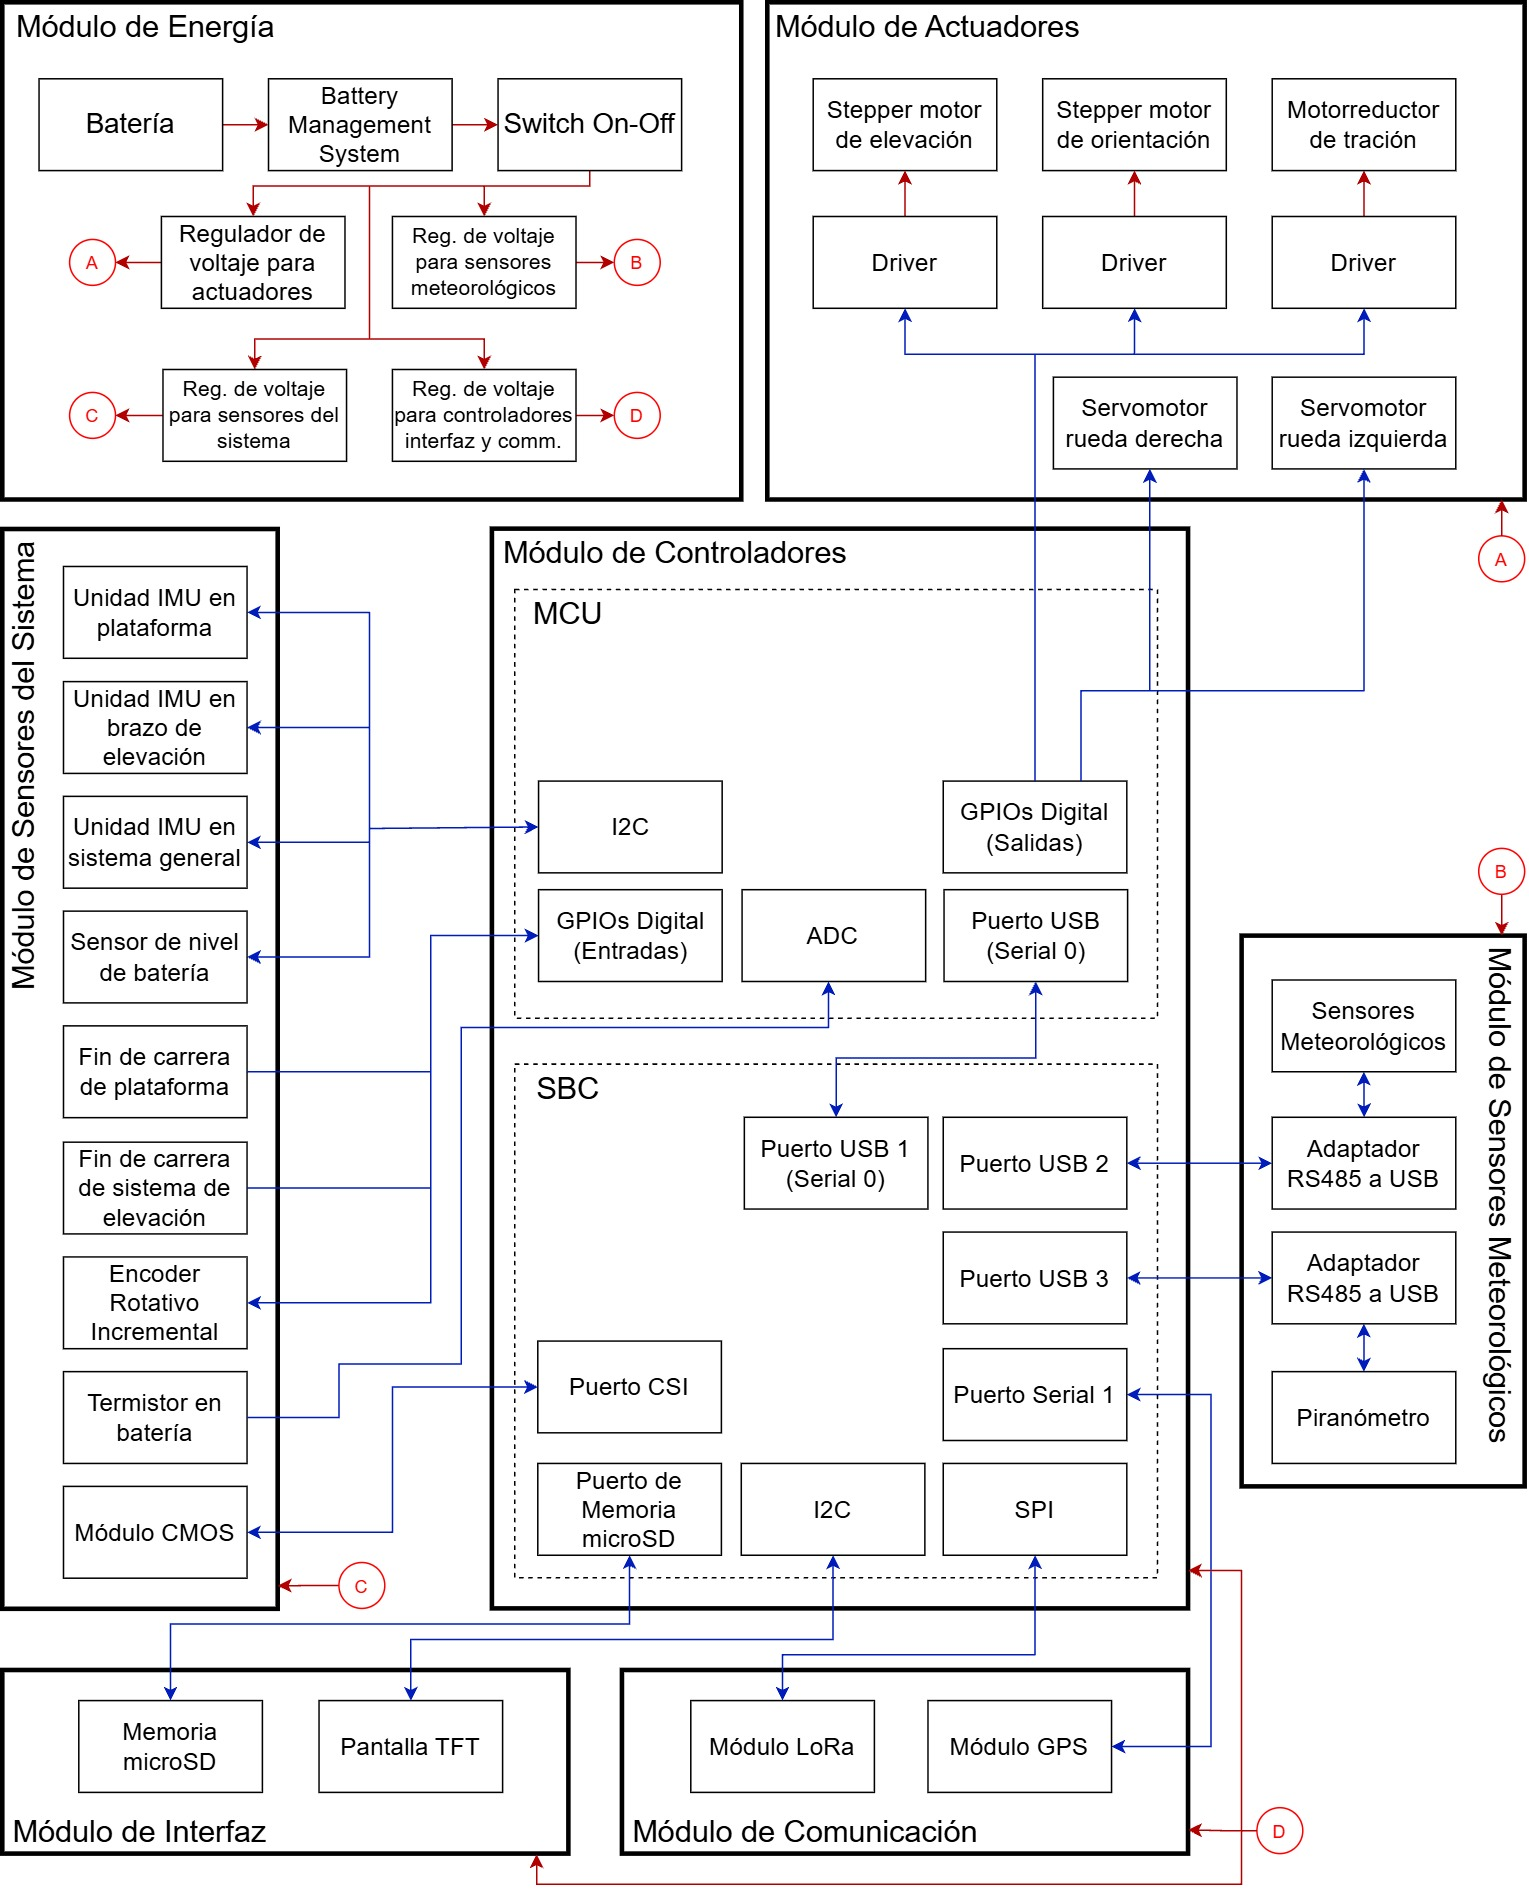
\includegraphics[width=\textwidth]{Recursos/Imagenes/ImagenesDisenoElectronico/DiagramaBloquesTFC1_v3.jpg} \par\medskip
    \raggedright
    \footnotesize \textit{Nota.} Elaboración propia.
    \label{fig:DiagramaBloques}
\end{figure}

\end{document}